\chapter{User-defined functions}
\label{chap:functions}

\section{Defining a function}
\label{func-define}

Since version 1.3.3, \app{gretl} has contained a mechanism for
defining functions in the context of a script.  This functionality has
been through some changes in search of a stable and extensible
framework.  We believe that the version present in \app{gretl} 1.6.1
should provide a good basis for future development.

Functions must be defined before they are called.  The syntax for
defining a function looks like this
    
\begin{code}
function function-name(parameters)
   function body
end function
\end{code}

\textsl{function-name} is the unique identifier for the function.
Names must start with a letter. They have a maximum length of 31
characters; if you type a longer name it will be truncated.  Function
names cannot contain spaces.  You will get an error if you try to
define a function having the same name as an existing \app{gretl}
command.

The \textsl{parameters} for a function are given in the form of a
comma-separated list.  Parameters can be of any of the types shown
below.

\begin{center}
\begin{tabular}{ll}
\multicolumn{1}{c}{Type} & 
\multicolumn{1}{c}{Description} \\ [4pt]
\texttt{bool}   & scalar variable acting as a Boolean switch \\
\texttt{int}    & scalar variable acting as an integer  \\
\texttt{scalar} & scalar variable \\
\texttt{series} & data series \\
\texttt{list}   & named list of series \\
\texttt{matrix} & named matrix or vector \\
\texttt{string} & named string or string literal 
\end{tabular}
\end{center}

Each element in the listing of parameters must include two terms: a
type specifier, and the name by which the parameter shall be known
within the function.  An example follows:
%    
\begin{code}
function myfunc(series y, list xvars, bool verbose)
\end{code}

Each of the type-specifiers, with the exception of \texttt{list} and
\texttt{string}, may be modified by prepending an asterisk to the
associated parameter name, as in
%    
\begin{code}
function myfunc(series *y, scalar *b)
\end{code}

The meaning of this modification is explained below (see section
\ref{funscope}); it is related to the use of pointer arguments in the
C programming language.  In addition, parameters may be modified by
the tag \texttt{const} (again, see \ref{funscope}).

\subsection{Function parameters: optional refinements}

Besides the required elements mentioned above, the specification of a
function parameter may include some additional fields.

For a parameter of type \texttt{scalar} or \texttt{int}, a
\textsl{minimum}, \textsl{maximum} and \textsl{default} value may be
specified.  These values should directly follow the name of the
parameter, enclosed in square brackets and with the individual
elements separated by colons.  For example, suppose we have an integer
parameter \texttt{order} for which we wish to specify a minimum of 1,
a maximum of 12, and a default of 4.  We can write
%    
\begin{code}
int order[1:12:4]
\end{code} 
%
If you wish to omit any of the three specifiers, leave the
corresponding field empty.  For example \texttt{[1::4]} would specify
a minimum of 1 and a default of 4 while leaving the maximum
unlimited.  

For a parameter of type \texttt{bool}, you can specify a default of
1 (true) or 0 (false), as in
%    
\begin{code}
bool verbose[0]
\end{code} 
%

Finally, for a parameter of any type you can append a short
\textsl{descriptive string}.  This will show up as an aid to the user
if the function is packaged (see section~\ref{sec:func-packages}
below) and called via \app{gretl}'s graphical interface.  The string
should be enclosed in double quotes, and inserted before the comma
that precedes the following parameter (or the closing right
parenthesis of the function definition, in the case of the last
parameter), as illustrated in the following example.

\begin{code}
function myfun (series y "dependent variable", 
                series x "independent variable")
\end{code} 

\subsection{Void functions}

You may define a function that has no parameters (these are called
``routines'' in some programming languages).  In this case,  
use the keyword \texttt{void} in place of the listing of parameters:
%    
\begin{code}
function myfunc2(void)
\end{code}


\subsection{The function body}
   
The \textsl{function body} is composed of \app{gretl} commands, or
calls to user-defined functions (that is, function calls may be
nested).  A function may call itself (that is, functions may be
recursive). While the function body may contain function calls, it may
not contain function definitions.  That is, you cannot define a
function inside another function.  For further details, see
section~\ref{func-details}.


\section{Calling a function}
\label{func-call}

A user function is called by typing its name followed by zero or more
arguments enclosed in parentheses.  If there are two or more arguments
these should be separated by commas.  

There are automatic checks in place to ensure that the number of
arguments given in a function call matches the number of parameters,
and that the types of the given arguments match the types specified in
the definition of the function.  An error is flagged if either of
these conditions is violated.  One qualification: allowance is made
for omitting arguments at the end of the list, provided that default
values are specified in the function definition.  To be precise, the
check is that the number of arguments is at least equal to the number
of \textit{required} parameters, and is no greater than the total
number of parameters.

A scalar, series or matrix argument to a function may be given either
as the name of a pre-existing variable or as an expression which
evaluates to a variable of the appropriate type.  Scalar arguments may
also be given as numerical values.  List arguments must be specified
by name.

The following trivial example illustrates a function call that
correctly matches the function definition.
    
\begin{code}
# function definition
function ols_ess(series y, list xvars)
  ols y 0 xvars --quiet
  scalar myess = $ess
  printf "ESS = %g\n", myess
  return scalar myess
end function
# main script
open data4-1
list xlist = 2 3 4
# function call (the return value is ignored here)
ols_ess(price, xlist)
\end{code}

The function call gives two arguments: the first is a data series
specified by name and the second is a named list of regressors.  Note
that while the function offers the variable \verb+myess+ as a return
value, it is ignored by the caller in this instance.  (As a side note
here, if you want a function to calculate some value having to do with
a regression, but are not interested in the full results of the
regression, you may wish to use the \option{quiet} flag with the
estimation command as shown above.)
    
A second example shows how to write a function call that assigns
a return value to a variable in the caller:
    
\begin{code}
# function definition
function get_uhat(series y, list xvars)
  ols y 0 xvars --quiet
  series uh = $uhat
  return series uh
end function
# main script
open data4-1
list xlist = 2 3 4
# function call
series resid = get_uhat(price, xlist)
\end{code}

\section{Deleting a function}
\label{func-del}

If you have defined a function and subsequently wish to clear it out
of memory, you can do so using the keywords \texttt{delete} or
\texttt{clear}, as in

\begin{code}
function myfunc delete
function get_uhat clear
\end{code}

Note, however, that if \texttt{myfunc} is already a defined function,
providing a new definition automatically overwrites the previous one,
so it should rarely be necessary to delete functions explicitly.

\section{Function programming details}
\label{func-details}

\subsection{Variables versus pointers}
\label{funscope}

Series, scalar, and matrix arguments to functions can be passed in two
ways: ``as they are'', or as pointers. For example, consider the
following:
\begin{code}
function triple1(series x)
  series ret = 3*x
  return series ret
end function
  
function triple2(series *x)
  series ret = 3*x
  return series ret
end function
\end{code}

These two functions are nearly identical (and yield the same result);
the only difference is that you need to feed a series into
\texttt{triple1}, as in \texttt{triple1(myseries)}, while
\texttt{triple2} must be supplied a \emph{pointer} to a series, as in
\texttt{triple2(\&myseries)}. 

Why make the distinction, then? There are two main reasons for doing
so: modularity and performance.

By modularity we mean the insulation of a function from the rest of
the script which calls it.  One of the many benefits of this approach
is that your functions are easily reusable in other contexts.  To
achieve modularity, \emph{variables created within a function are
  local to that function, and are destroyed when the function exits},
unless they are made available as return values and these values are
``picked up'' or assigned by the caller.
    
In addition, functions do not have access to variables in ``outer
scope'' (that is, variables that exist in the script from which the
function is called) except insofar as these are explicitly passed to
the function as arguments.

By default, when a variable is passed to a function as an argument,
what the function actually ``gets'' is a \emph{copy} of the outer
variable, which means that the value of the outer variable is not
modified by whatever goes on inside the function.  But the use of
pointers allows a function and its caller to ``cooperate'' such that
an outer variable can be modified by the function.  In effect, this
allows a function to ``return'' more than one value (although only one
variable can be returned directly --- see below).  The parameter in
question is marked with a prefix of \texttt{*} in the function
definition, and the corresponding argument is marked with the
complementary prefix \verb+&+ in the caller.  For example,
%
\begin{code}
function get_uhat_and_ess(series y, list xvars, scalar *ess)
  ols y 0 xvars --quiet
  ess = $ess
  series uh = $uhat
  return series uh
end function
# main script
open data4-1
list xlist = 2 3 4
# function call
scalar SSR
series resid = get_uhat_and_ess(price, xlist, &SSR)
\end{code}
%
In the above, we may say that the function is given the \emph{address}
of the scalar variable \texttt{SSR}, and it assigns a value to that
variable (under the local name \texttt{ess}).  (For anyone used to
programming in C: note that it is not necessary, or even possible, to
``dereference'' the variable in question within the function using the
\texttt{*} operator.  Unembellished use of the name of the variable is
sufficient to access the variable in outer scope.)

An ``address'' parameter of this sort can be used as a means of
offering optional information to the caller.  (That is, the
corresponding argument is not strictly needed, but will be used if
present).  In that case the parameter should be given a default value
of \texttt{null} and the the function should test to see if the caller
supplied a corresponding argument or not, using the built-in function
\texttt{isnull()}.  For example, here is the simple function shown
above, modified to make the filling out of the \texttt{ess} value
optional.
%
\begin{code}
function get_uhat_and_ess(series y, list xvars, scalar *ess[null])
  ols y 0 xvars --quiet
  if !isnull(ess) 
     ess = $ess
  endif
  series uh = $uhat
  return series uh
end function
\end{code}
%
If the caller does not care to get the \texttt{ess} value, it should
use \texttt{null} in place of a real argument:
%
\begin{code}
series resid = get_uhat_and_ess(price, xlist, null)
\end{code}

Using pointers may also be useful for optimizing performance: even if
a variable is not modified inside the function, it may be a good idea
to pass it as a pointer if it occupies a lot of memory. Otherwise, the
time \app{gretl} spends transcribing the value of the variable to the
local copy may be non-negligible, compared to the time the function
spends doing the job it was written for.

Example \ref{ex:perf-pointers} takes this to the extreme.  We define
two functions which return the number of rows of a matrix (a pretty
fast operation).  One function gets a matrix as argument, the other
one a pointer to a matrix.  The two functions are evaluated on a
matrix with 2000 rows and 2000 columns; on a typical system,
floating-point numbers take 8 bytes of memory, so the space occupied
by the matrix is roughly 32 megabytes.

Running the code in example \ref{ex:perf-pointers} will produce output
similar to the following (the actual numbers depend on the
machine you're running the example on):
\begin{code}
Elapsed time: 
	without pointers (copy) = 3.66 seconds,
	with pointers (no copy) = 0.01 seconds.
\end{code}

\begin{script}[htbp]
  \caption{Performance comparison: values versus pointer}
  \label{ex:perf-pointers}
  \begin{scode}
function a(matrix X)
  r = rows(X)
  return scalar r
end function

function b(matrix *X)
  r = rows(X)
  return scalar r
end function

nulldata 10
set echo off
set messages off
X = zeros(2000,2000)
r = 0

set stopwatch
loop 100
  r = a(X)
end loop
fa = $stopwatch

set stopwatch
loop 100
  r = b(&X)
end loop
fb = $stopwatch

printf "Elapsed time:\n\
\twithout pointers (copy) = %g seconds,\n\
\twith pointers (no copy) = %g seconds.\n", fa, fb 
\end{scode}
%$
\end{script}

\subsection{List arguments}

The use of a named list as an argument to a function gives a means of
supplying a function with a set of variables whose number is unknown
when the function is written --- for example, sets of regressors or
instruments.  Within the function, the list can be passed on to
commands such as \texttt{ols}, or it can be ``unpacked'' using a
\texttt{foreach} loop construct.  For example, suppose you have a list
\texttt{X} and want to calculate the standard deviation of each
variable in the list:
%
\begin{code}
loop foreach i X
   scalar sd_$i = sd($i)
end loop
\end{code}

When a named list of variables is passed to a function, the function
is provided with a copy of the list.  The variables referenced in the
list are, however, made directly accessible to the function, in a
similar manner to the case where a scalar or series argument is passed
in ``pointer'' form, as discussed above.  Passing a list is therefore
another means of allowing a function to do more in the way of
modifying data at the level of the caller than simply offering a
return value.  If the variables will \textit{not} be modified inside
the function, it is a good idea to flag this fact using the
\texttt{const} modifier in the listing of parameters:
%
\begin{code}
function myfunc (scalar y, const list X)
\end{code}
%
When a list is marked \texttt{const}, any attempt to rename, delete
or overwrite the original values of the variables in the list will
generate an error.

If a list argument to a function is optional, this should be indicated
by appending a default value of \texttt{null}, as in
%
\begin{code}
function myfunc (scalar y, list X[null])
\end{code}
%
In that case, if the caller gives \texttt{null} as the list argument
then the named list \texttt{X} inside the function will be empty.
This possibility can be detected using the \texttt{nelem()} function,
which returns 0 for an empty list.  (This mechanism can also be used
to check whether a named, but empty, list was supplied as an
argument.)

\subsection{String arguments}

String arguments can be used, for example, to provide flexibility in
the naming of variables created within a function.  In the following
example the function \texttt{movavg} returns a list containing two
moving averages constructed from an input series, with the names of
the newly created variables governed by the string argument.
%
\begin{code}
function movavg (series y, string vname)
   series @vname_2 = (y+y(-1)) / 2
   series @vname_4 = (y+y(-1)+y(-2)+y(-3)) / 4
   list retlist = @vname_2 @vname_4
   return list retlist
end function

open data9-9
list malist = movavg(nocars, "nocars")
print malist --byobs
\end{code}
%
The last line of the script will print two variables named
\verb|nocars_2| and \verb|nocars_4|.  For details on the handling of
named strings, see chapter~\ref{chap-persist}.


\subsection{Retrieving the names of arguments}

The variables given as arguments to a function are known inside the
function by the names of the corresponding parameters.  For example,
within the function whose signature is
%
\begin{code}
function somefun (series y)
\end{code}
%
we have the series known as \texttt{y}.  In may be useful, however, to
be able to determine the names of the variables provided as arguments.
This can be done using the function \texttt{argname}, which takes the
name of a function parameter as its single argument and returns a
string.  Here is a simple illustration:
%
\begin{code}
function namefun (series y)
  printf "the series given as 'y' was named %s\n", argname(y)
end function

open data9-7
namefun(QNC)
\end{code}
%
This produces the output
%
\begin{code}
the series given as 'y' was named QNC
\end{code}

It should be noted that this will not always work: the arguments given
to functions may be anonymous variables, created on the fly, as in
\texttt{somefun(log(QNC))} or \texttt{somefun(CPI/100)}.  In that case
the \textsf{argname} function returns an empty string.  Function
writers who wish to make use of this facility should check the return
from \texttt{argname} using the \texttt{isstring()} function, which
returns 1 for a non-empty string, 0 otherwise.


\subsection{Return values}

Functions can return nothing (just printing a result, perhaps), or
they can return a single variable --- a scalar, series, list, matrix
or string.  The return value, if any, is specified via a statement
within the function body beginning with the keyword \verb+return+,
followed by a type specifier and the name of a variable (as in the
listing of parameters).  There can be only one such statement.  An
example of a valid return statement is shown below:
%    
\begin{code}
return scalar SSR
\end{code}
%
Having a function return a list is one way of permitting the
``return'' of more than one variable.  That is, you can define several
variable inside a function and package them as a list; in this case
they are not destroyed when the function exits.  Here is a simple
example, which also illustrates the possibility of setting the
descriptive labels for variables generated in a function.
%    
\begin{code}
function make_cubes (list xlist)
   list cubes = null
   loop foreach i xlist --quiet
      series $i3 = $i^3
      setinfo $i3 -d "cube of $i"
      list cubes += $i3
    end loop
    return list cubes
end function

open data4-1
list xlist = price sqft
list cubelist = make_cubes(xlist)
print xlist cubelist --byobs
labels
\end{code}
%$

Note that the \verb+return+ statement does \emph{not} cause the
function to return (exit) at the point where it appears within the
body of the function. Rather, it specifies which variable is available
for assignment when the function exits, and a function exits only when
(a) the end of the function code is reached, (b) a \app{gretl} error
occurs, or (c) a \verb+funcerr+ statement is reached.

The \verb+funcerr+ keyword, which may be followed by a string enclosed
in double quotes, causes a function to exit with an error flagged.  If
a string is provided, this is printed on exit, otherwise a generic
error message is printed.  This mechanism enables the author of a
function to pre-empt an ordinary execution error and/or offer a more
specific and helpful error message.  For example,
%
\begin{code}
if nelem(xlist) = 0
   funcerr "xlist must not be empty"
end if
\end{code}
    

\subsection{Error checking}

When gretl first reads and ``compiles'' a function definition there is
minimal error-checking: the only checks are that the function name is
acceptable, and, so far as the body is concerned, that you are not
trying to define a function inside a function (see Section
\ref{func-define}). Otherwise, if the function body contains invalid
commands this will become apparent only when the function is called,
and its commands are executed.


\subsection{Printing of output}

The usual mechanism whereby \app{gretl} echos commands, and reports on
the creation of new variables, is suppressed by default when a
function is being executed.  If you want to turn this on (for example,
for the purpose of debugging function code), you can issue one or both
of the following commands inside the function:
%
\begin{code}
set echo on
set messages on
\end{code}

\section{Function packages}
\label{sec:func-packages}

As of \app{gretl} 1.6.0, there is a mechanism to package functions and
make them available to other users of \app{gretl}.  This is currently
experimental, but here is a walk-through of the process.

\subsection{Load a function in memory}

There are several ways to load a function:

\begin{itemize}
\item If you have a script file containing function definitions, open
  that file and run it.
\item Create a script file from scratch.  Include at least one
  function definition, and run the script.
\item Open the GUI console and type a function definition
  interactively.  This method is not particularly recommended; you are
  probably better composing a function non-interactively.
\end{itemize}

For example, suppose you decide to package a function that returns the
percentage change of a time series. Open a script file and type
\begin{code}
function pc(series y "Series to process")
  series foo = diff(y)/y(-1)
  return series foo
end function
\end{code}
In this case, we have appended a string to the function
argument, as explained in section \ref{func-define}, so to make our
interface more informative. This is not obligatory: if you omit the
descriptive string, \app{gretl} will supply a predefined one.

\begin{figure}[htbp]
  \centering
  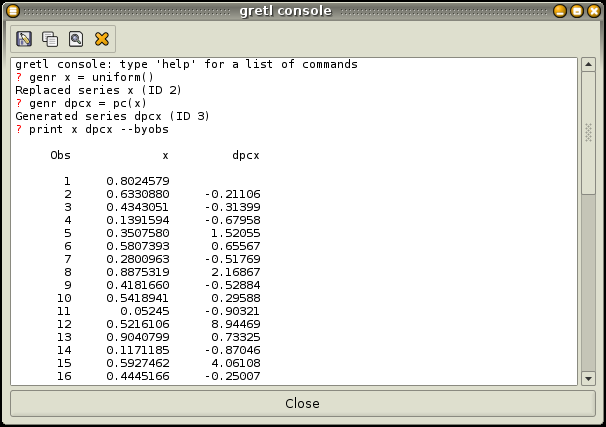
\includegraphics[scale=0.5]{figures/func_check}
  \caption{Output of function check}
  \label{fig:func_check}
\end{figure}

Now run your function. You may want to make sure your function works
properly by running a few tests. For example, you may open the console
and type

\begin{code}
genr x = uniform()
genr dpcx = pc(x)
print x dpcx --byobs
\end{code}

You should see something similar to figure \ref{fig:func_check}. The
function seems to work ok. Once your function is debugged, you
may proceed to the next stage.

\subsection{Create a package}

Start the GUI program and take a look at the ``File, Function files'' menu.
This menu contains four items: ``On local machine'', ``On server'', ``Edit
package'', ``New package''.

Select ``New package'' (the command will return an error message,
unless at least one user-defined function is currently loaded in
memory --- see the previous point); in the first dialog you get to
select:

\begin{itemize}
\item A public function to package.
\item Zero or more ``private'' helper functions.
\end{itemize}

Public functions are directly available to users; private functions are
part of the ``behind the scenes'' mechanism in a function package.

\begin{figure}[htbp]
  \centering
  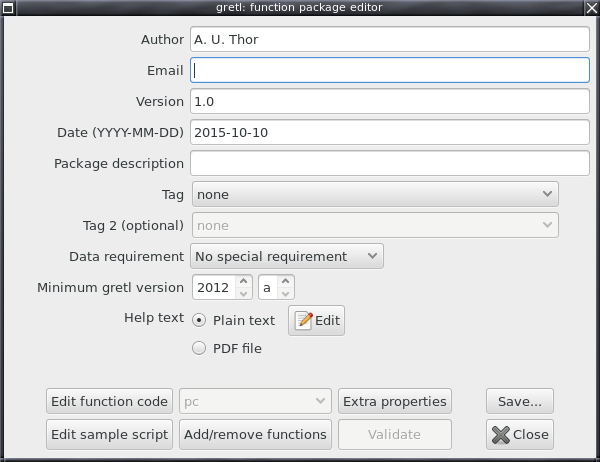
\includegraphics[scale=0.5]{figures/package_editor}
  \caption{The package editor window}
  \label{fig:package_editor}
\end{figure}

On clicking ``OK'' a second dialog should appear (see figure
\ref{fig:package_editor}), where you get to enter the package
information (currently, author, version, date, and a short
description).  You also get to enter help text for the public
interface.  You have a further chance to edit the code of the
functions to be packaged, by selecting them from the drop-down
selector and clicking on ``Edit function code''. Finally, you can
choose to upload the package on gretl's server as soon as it is saved,
by checking the relevant checkbox.

Clicking ``OK'' in this dialog leads you to a File Save dialog.  All
being well, this should be pointing towards a directory named
\texttt{functions}, either under the \app{gretl} system directory (if
you have write permission on that) or the \app{gretl} user directory.
This is the recommended place to save function package files, since
that is where the program will look in the special routine for opening
such files (see below).

Needless to say, the menu command ``File, Function files, Edit package''
allows you to edit again a local function package.

\vspace{6pt}

A word on the file you just saved.  By default, it will have a
\texttt{.gfn} extension.  This is a ``function package'' file: unlike
an ordinary \app{gretl} script file, it is an XML file containing both
the function code and the extra information entered in the packager.
Hackers might wish to write such a file from scratch rather than using
the GUI packager, but most people are likely to find it awkward.  Note
that XML-special characters in the function code have to be escaped,
e.g.\ \texttt{\&} must be represented as \texttt{\&amp;}.  Also, some
elements of the function syntax differ from the standard script
representation: the parameters and return values (if any) are
represented in XML.  Basically, the function is pre-parsed, and ready
for fast loading using \textsf{libxml}.

\vspace{6pt}

\subsection{Load a package}

Why package functions in this way?  To see what's on offer so far, try
the next phase of the walk-through.

Close gretl, then re-open it.  Now go to ``File, Function files, On
local machine''. If the previous stage above has gone OK, you should
see the file you packaged and saved, with its short description.  If
you click on ``Info'' you get a window with all the information gretl
has gleaned from the function package.  If you click on the ``View
code'' icon in the toolbar of this new window, you get a script view
window showing the actual function code. Now, back to the ``Function
packages'' window, if you click on the package's name, the functions
are loaded into gretl, ready to be called by clicking on the ``Call''
button.

After loading the function(s) from the package, open the GUI console.
Try typing \texttt{help foo}, replacing \texttt{foo} with the name of
the public interface from the loaded function package: if any help text
was provided for the function, it should be presented.

In a similar way, you can browse and load the function packages
available on the \app{gretl} server, by selecting ``File, Function
files, On server''.

Once your package is installed on your local machine, you can use the
function it contains via the graphical interface as described above,
or by using the CLI, namely in a script or through the console. In the
latter case, you load the function via the \texttt{include} command,
specifying the package file as the argument, complete with the
\texttt{.gfn} extension.

\begin{figure}[htbp]
  \centering
  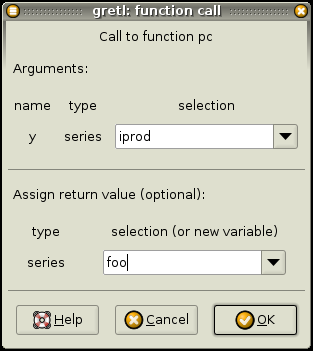
\includegraphics[scale=0.5]{figures/function_call}
  \caption{Using your package}
  \label{fig:function_call}
\end{figure}

To continue with our example, load the file \texttt{np.gdt} (supplied
with \app{gretl} among the sample datasets). Suppose you want to
compute the rate of change for the variable \texttt{iprod} via your
new function and store the result in a series named \texttt{foo}.

Go to ``File, Function files, On local machine''.  You will be shown a
list of the installed packages, including the one you have just
created. If you select it and click on ``Execute'' (or double-click on
the name of the function package), a window similar to the one shown
in figure \ref{fig:function_call} will appear.  Notice that the
description string ``Series to process'', supplied with the function
definition, appears to the left of the top series chooser.

Click ``Ok'' and the
series \texttt{foo} will be generated (see figure \ref{fig:iprod_pc}).
You may have to go to ``Data, Refresh data'' in order to have your new
variable show up in the main window variable list (or just press the
``r'' key).

\begin{figure}[htbp]
  \centering
  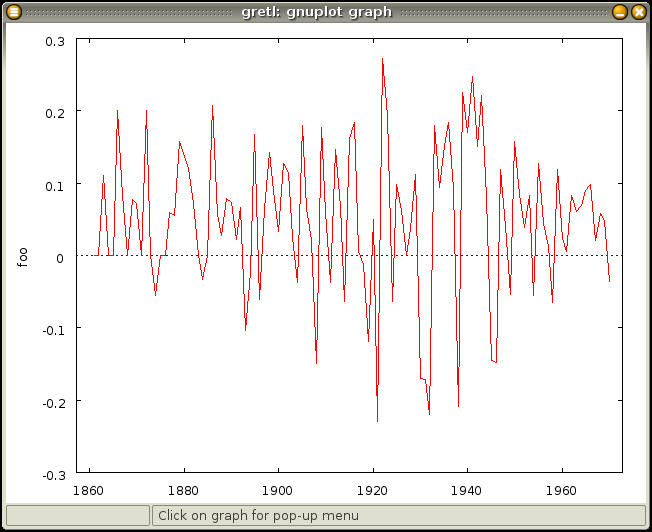
\includegraphics[scale=0.5]{figures/iprod_pc}
  \caption{Percent change in industrial production}
  \label{fig:iprod_pc}
\end{figure}

Alternatively, the same could have been accomplished by the script
\begin{code}
include pc.gfn
open np
foo = pc(iprod)
\end{code}

%%% Local Variables: 
%%% mode: latex
%%% TeX-master: "gretl-guide"
%%% End: 

